\chapter{Phase Imaging using Coded Illumination}\label{ch:phase}

Light is a propagating wave, having a velocity, wavelength (color), amplitude, and phase. As a single ray of light reaches an interface, it can be absorbed (reduced in amplitude) or undergo a change in phase through reflection, refraction, or diffraction based on the material properties and geometry of the object. Measuring this electromagnetic field at the sample plane is the primary goal of an imaging system; however, the current camera technology can only measure the amplitude of this complex field due to the relatively slow speed of silicon-based computing systems compared to the frequency of electromagnetic waves at optical wavelengths. For example, a coherent wavefront with wavelength $530nm$ traveling in air will have an oscillation period of approximately 1.76 femtoseconds ($1.76 \times 10^{-15} s$), which would need to be sampled at a rate of 1.13 petahertz ($1.13 \times 10^{15} Hz$) to sample the waveform at the Nyquist rate. Practical limitations of silicon-based computers limit their clock speeds of around 10 GHz ($10^9 Hz$), making it impossible to measure an optical wavefront by directly sampling it electronically. Instead, conventional cameras measure hundreds of thousands of periods of a waveform, averaging these periods to capture the intensity of the wavefront, which contains no direct phase information (although the phase of a wavefront can be indirectly inferred using camera hardware employing interferometric~\cite{phasics, platt2001history} or geometric~\cite{Ng2005} methods).

Mathematically, the process of measuring the intensity of a wavefront described as taking the magnitude of the complex field $I =|\vec{E}|^2 =|\vec{A}e^{i\vec{\phi}}|^2 = \vec{A}^2$ where $\vec{A}$ is the amplitude of a wave and $\vec{\phi}$ is the phase of the wavefront in this phasor notation. Phase is related to the mechanical geometry of the cell by the relationship $\vec{\phi} = \frac{2\pi}{\lambda} \vec{n} \vec{d}$, where $\lambda$ is the system wavelength, $\vec{n}$ is the refractive index change, and $\vec{d}$ is the thickness of the object.

This loss of phase information is particularly problematic for imaging aqueous samples, such as biological cells. To counter this, biologists often apply chemical stains to add absorption contrast artificially, but this process is cumbersome and can modify the micro-environment in significant ways. Optical phase imaging methods such as Differential Interference Contrast (DIC)\cite{smithDIC} and Zernike Phase Contrast (PhC) \cite{zernike1955discovered} were developed to provide phase contrast, which is a mix phase and amplitude of the wavefront and requires no chemical staining. These methods have since become widely adopted due to their simplicity and ability to reveal phase information in aqueous samples without adding additional contrast agents (stains).

\section{Quantitative Phase Imaging}
Quantitative Phase Imaging (QPI) involves recovering the complete amplitude and phase, or complex field, of a sample. In contrast to \emph{qualitative} phase imaging methods, such as Zernike phase contrast and DIC, \emph{quantitative} methods recover the phase delay caused by the sample, decoupled from absorption information. Modifications of PhC~\cite{yun2010system} and DIC~\cite{CuiYangTearney2011} can make these setups quantitative, at a cost of requiring multiple images. More commonly, QPI methods use interferometry with coherent illumination and a reference beam~\cite{Wang2011, Popescu2006, Bhaduri:12}, making them expensive and sensitive to misalignment and vibrations.

In optical microscopy, low cost and low-complexity methods which require little hardware modification are often preferred to more complex interferometric methods for practical reasons such as cost and calibration limitations. Through-focus phase retrieval~\cite{waller2010transport, Petruccelli:12, Jingshan14GPTIE} recovers the complex field using defocused intensity measurements of the sample by solving the transport of intensity (TIE) equation. TIE-based phase imaging has also been extended to use partially-coherent sources, which provides higher resolution than under coherent illumination~\cite{JingsanSourceRecovery2016}. The TIE equation is non-linear, however, and requires a second-order solver and phase unwrapping algorithm to accurately recover the full complex field.

Most quantitative phase imagine methods require the user to capture multiple images to facilitate phase recovery. Amongst the wide array of existing QPI methods only a small number are single-shot, since disambiguating amplitude and phase from a single-measurement is an ill-posed problem. Off-axis holography interferes the sample beam with a tilted reference beam, then recovers phase by Fourier filtering~\cite{Witte:12}. Parallel phase-shifting can spatially multiplex several holograms within a single exposure via an array of polarizers~\cite{2004singleshotPSDH}. And single-shot QPI add-ons based on amplitude gratings work with commercial microscopes, replacing the traditional camera module~\cite{phasics,bon2012method}. Another add-on option uses two cameras to capture defocused images which can then be used to solve the transport of intensity equation (TIE)~\cite{allman2005optical}. Alternatively, if chromatic aberrations are large enough, they can enable single-shot color TIE~\cite{gross:14, wallerColorTIE} without any hardware changes.

In the remaining sections of this chapter, we describe a quantitative phase imaging method which uses a programmable partially-coherent light source to perform quantitative phase imaigng, and demonstrate a single-shot variant which uses a color-multiplexing and inexpensive 3D-printed inserts to enable high-speed recovery of the complex field of a sample.

\section{Differential Phase Contrast}
Differential Phase Contrast (DPC)~\cite{Hamilton1984a,mehta2009quantitative,Tian14,tian2015quantitative} is a partially coherent QPI technique that uses asymmetric illumination to shift the sample's spectrum in Fourier space, revealing phase information in a weak object. While raw DPC measurements provide phase contrast which is similar to DIC contrast, the DPC method provides a linearization of the image formation model which can be inverted using a single-step deconvolution process (Quantitative DPC)~\cite{mehta2009quantitative,tian2015quantitative}. Quantitative DPC recovers both amplitude and phase with resolution up to the incoherent resolution limit ($2\times$ better than coherent methods). Practically, the illumination switching can be done quickly and at low cost with an LED array~\cite{Tian14,zijiMulti,tian2015quantitative}. At least two complementary source patterns are required, but generally 3-4 patterns (top, bottom, left, right half-circles) are used to avoid missing spatial frequencies. The DPC method was recently extended to color multiplexing~\cite{lee2015color}, where the 4 source patterns were encoded into two images by using a color camera in combination with a color LED array. Similarly, color photometric stereo has been used for retrographic surface profiling of large objects using off-axis color illumination in reflection mode~\cite{johnson2009retrographic}.

\begin{figure}[h]
\centering
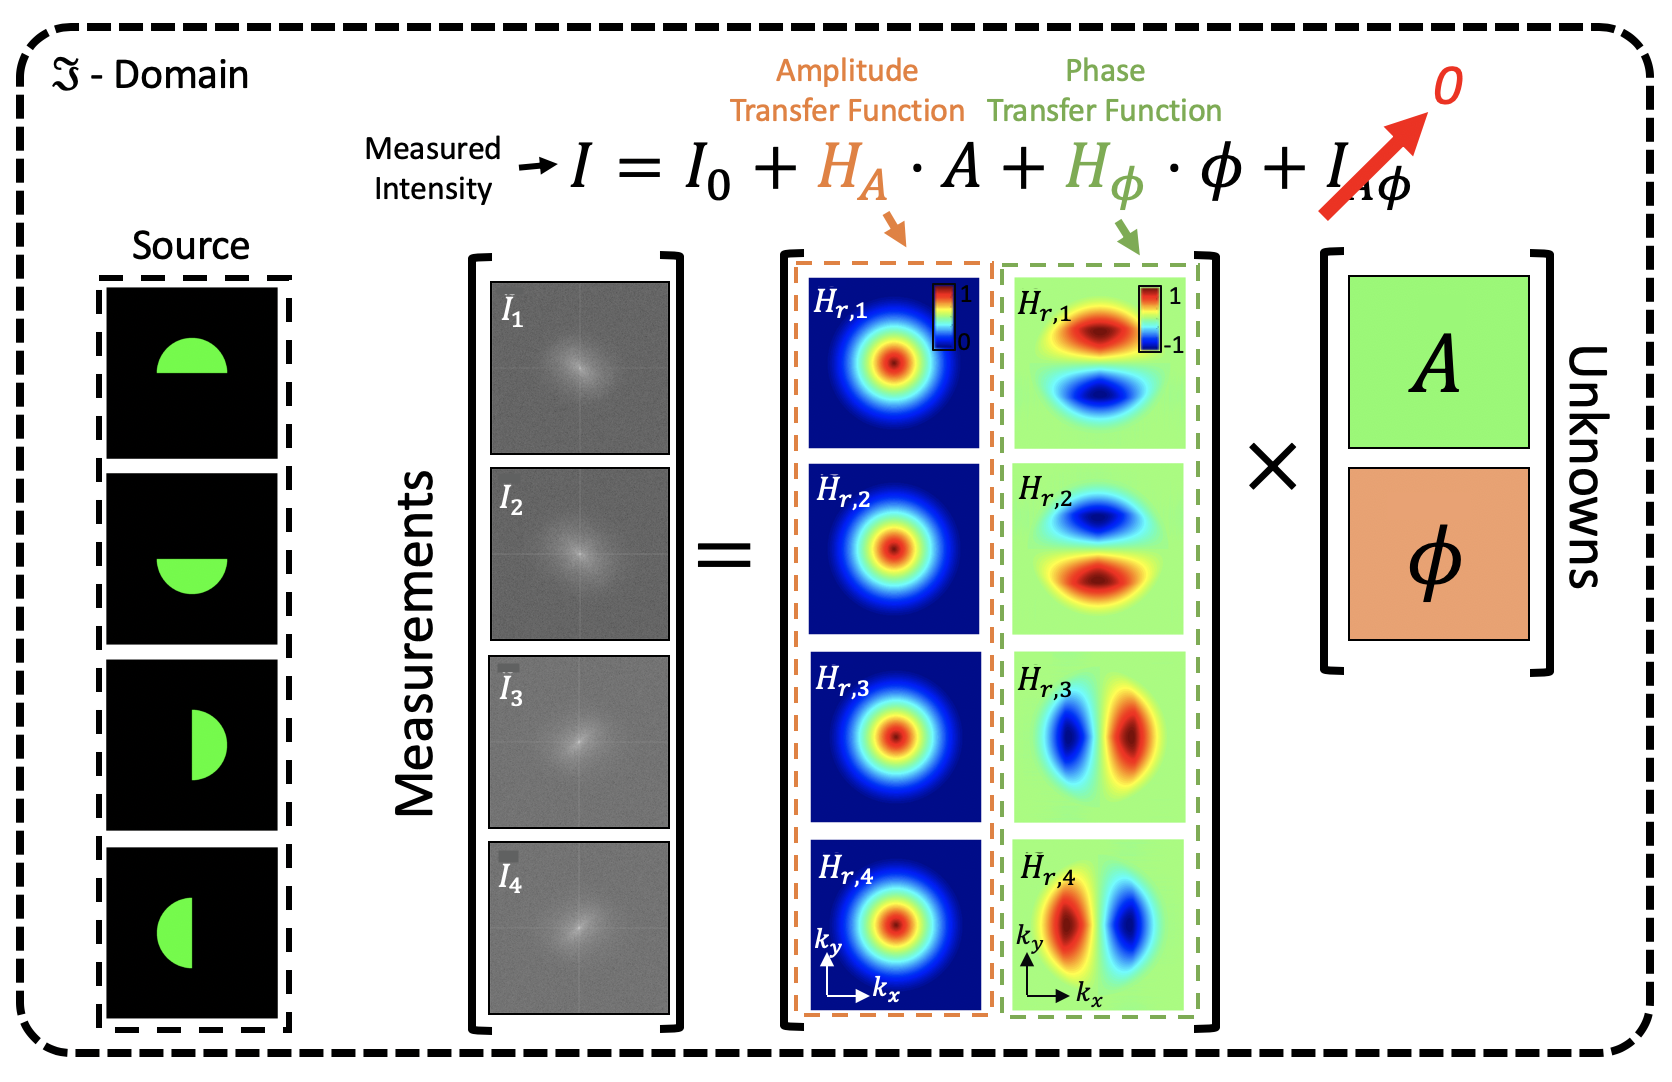
\includegraphics[width=1\textwidth]{figures/fig_phase_dpc_transfer.png}
\caption{\label{fig:dpc_transfer} Example transfer functions for typical half-circle illumination patterns.}
\end{figure}

\subsubsection{Forward model}
\label{sec:forward}
The geneal image formation model for a sample illuminated under a partially-coherent source is defined as the sum of many coherent forward models~\cite{mehta2009quantitative}:
\begin{equation}
I = \sum_i^N |\vec{P} * \vec{O}e^{-i2\pi \frac{\sin{\theta}_i}{\lambda} \vec{r}}|^2
\end{equation}

\noindent where $N$ sources illuminating from angles $\theta_i$ with wavelength $\lambda$ illuminate an object $\vec{O}$ which is then
 filtered by a pupil $\vec{P}$, having spatial coordinates $\vec{r}$. In general, this model is nonlinear and difficult to invert directly. DPC employs a linearized forward model to describe the intensity images that result from a given complex-field. This linearization is achieved by making a weak phase assumption on the sample's complex-field and ignoring higher order (nonlinear) terms in the Taylor expansion of the complex-field, $\vec{E} = e^{\mathrm{i}\vec{\phi} -\vec{\mu}} \approx 1 - \vec{\mu} + \mathrm{i}\vec{\phi}$.
Under the same approximation, the Weak Object Transfer Functions (WOTFs) for absorption ($\tilde{\vec{H}}_{\mu}$) and phase ($\tilde{\vec{H}}_{\phi}$) can be derived~\cite{Claus2015, tian2015quantitative, Hamilton1984a} to linearly related to intensity measurements:

\begin{equation}
	\vec{I}(r) = \vec{I}_{0} +\vec{H}_{\mu}(r) * \vec{\mu}(r) + \mathrm{i}\cdot \vec{H}_{\phi}(r) * \vec{\phi}(r) + \vec{I}_{ss}
	\label{eq:wotf_2}
\end{equation}

\noindent Here, $r$ represents 2D real-space coordinates, $\vec{I}$ is the intensity measurement, $\vec{I}_0$ is the background signal, and $*$ denotes convolution. $\vec{I}_{ss}$ is the $2^{nd}$ order scatter-scatter term, which is assumed to be small and is ignored in the DPC algorithm. Eq.~\ref{eq:wotf_2} can also be represented in the Fourier domain:

\begin{equation}
	\vec{\tilde{I}}(r) = \vec{\tilde{I}}_{0} + \vec{\tilde{H}}_{\mu}(r) \cdot \vec{\tilde{\mu}}(r) + \mathrm{i}\cdot \vec{\tilde{H}}_{\phi}(r) \cdot \vec{\tilde{\phi}}(r) + \vec{\tilde{I}}_{ss}
	\label{eq:wotf_2_f}
\end{equation}

\noindent Here, $\tilde{\cdot}$ represents the Fourier transform of the measurements and sample amplitude ($\vec{\mu}$) and phase ($\vec{\phi}$). Given a known source ($\vec{S}$), and pupil function ($\vec{P}$) whose bandwidth is set by the objective numerical aperture (NA) and wavelength ($\lambda$), the WOTFs are~\cite{Claus2015,tian2015quantitative}:

\begin{equation}\label{WOTF_re}
\tilde{\vec{H}}_{\mu}(k) = \vec{\tilde{P}}(k) \star (\vec{\tilde{P}}(k)\cdot \vec{\tilde{S}}(k))+ (\vec{\tilde{P}}(k) \cdot \vec{\tilde{S}}(k)) \star \vec{\tilde{P}}(k)
\end{equation}

\begin{equation}\label{WOTF_im}
\tilde{\vec{H}}_{\phi} (k) = \vec{\tilde{P}}(k) \star (\vec{\tilde{P}}(k)\cdot \vec{\tilde{S}}(k))- (\vec{\tilde{P}}(k) \cdot \vec{\tilde{S}}(k)) \star \vec{\tilde{P}}(k),
\end{equation}

\noindent where $k$ represents Fourier-domain coordinates. Generally, multiple DPC measurements are acquired together, resulting in a series of measurements $\{\vec{y}_1, \vec{y}_2, \cdots \vec{y}_n\}$ and a stacked forward model based on one pair of $\tilde{\vec{H}}_{\phi}$ and $\tilde{\vec{H}}_{\mu}$ for each source:

\begin{equation}
    \label{eq:dpc_forward_model}
    \begin{bmatrix}\tilde{\vec{y}}_1 \\ \tilde{\vec{y}}_2 \\ \tilde{\vec{y}}_3\end{bmatrix} = \begin{bmatrix}\tilde{\vec{H}}_{\mu, 1} & \tilde{\vec{H}}_{\phi, 1}\\ \tilde{\vec{H}}_{\mu, 2} & \tilde{\vec{H}}_{\phi, 2} \\ \tilde{\vec{H}}_{\mu, 3} & \tilde{\vec{H}}_{\phi, 3}\end{bmatrix} \times \begin{bmatrix}\tilde{\vec{\mu}} \\ \tilde{\vec{\phi}}\end{bmatrix}
\end{equation}

\subsection{Phase Reconstruction}
Eq.~\ref{eq:dpc_forward_model} is linear and can be inverted using linear least squares~\cite{tian2015quantitative} to recover phase and absorption of the complex field. Due to nulls in the WOTFs, it is often prudent to add regularization (such as Tikhonov) to ensure noise is not amplified unnecessarily during the reconstruction process. With $m$ measurements and Tikhonov regularization parameters $\gamma_{\mu}$ and $\gamma_{\phi}$, the linearized complex field absorption ($\vec{\mu}$) and phase ($\vec{\phi}$) can be recovered using the following equations:

\begin{equation} \label{eq:Ha_inverse}
\mu = F^{-1}\left\{\frac{\left(\sum\limits_{m}|\tilde{\vec{H}}_{\phi,m}|^2+\gamma_{\phi}\right)\cdot\sum\limits_{m}\left(\tilde{\vec{H}}^*_{\mu,m}\cdot\tilde{\vec{I}}'_{m}\right)-\sum\limits_{m} \left ( \tilde{\vec{H}}^*_{\mu,m}\cdot\tilde{\vec{H}}_{\phi,m} \right ) \cdot\sum\limits_{m}\left(\tilde{\vec{H}}^*_{\phi,m}\cdot\tilde{\vec{I}}'_{m}\right)}{\left(\sum\limits_{m}|\tilde{\vec{H}}_{\mu,m}|^2+\gamma_{\mu}\right)\cdot\left(\sum\limits_{m}|\tilde{\vec{H}}_{\phi,m}|^2+\gamma_{\phi}\right) - \sum\limits_{m}\left(\tilde{\vec{H}}_{\mu,m}\cdot\tilde{\vec{H}}^*_{\phi,m}\right)\cdot\sum\limits_{m}\left(\tilde{\vec{H}}^*_{\mu,m}\cdot\tilde{\vec{H}}_{\phi,m}\right)} \right\}
\end{equation}

\begin{equation} \label{eq:Hp_inverse}
\phi = F^{-1}\left\{\frac{-\mathrm{i}\cdot\left[\left(\sum\limits_{m}|\tilde{\vec{H}}_{\mu,m}|^2+\gamma_{\mu}\right)\cdot\sum\limits_{m}\left(\tilde{\vec{H}}^*_{\phi,m}\cdot\tilde{\vec{I}}'_{m}\right)-\sum\limits_{m}\left(\tilde{\vec{H}}_{\mu,m}\cdot\tilde{\vec{H}}^*_{\phi,m}\right)\cdot\sum\limits_{m}\left(\tilde{\vec{H}}^*_{\mu,m}\cdot\tilde{\vec{I}}'_{m}\right)\right]}{\left(\sum\limits_{m}|\tilde{\vec{H}}_{\mu,m}|^2+\gamma_{\mu}\right)\cdot\left(\sum\limits_{m}|\tilde{\vec{H}}_{\phi,m}|^2+\gamma_{\phi}\right)-\sum\limits_{m}\left(\tilde{\vec{H}}_{\mu,m}\cdot\tilde{\vec{H}}^*_{\phi,m}\right)\cdot\sum\limits_{m} \left( \tilde{\vec{H}}^*_{\mu,m}\cdot\tilde{\vec{H}}_{\phi,m} \right )} \right\},
\end{equation}

\noindent For improved performance, other regularizers such as Total Variation (TV) regularization~\cite{osher2005iterative}, although many of these methods require iterative solvers such as FISTA~\cite{beck2009fast} which is slower than direct inversion.

\begin{figure}[tbh]
\centering
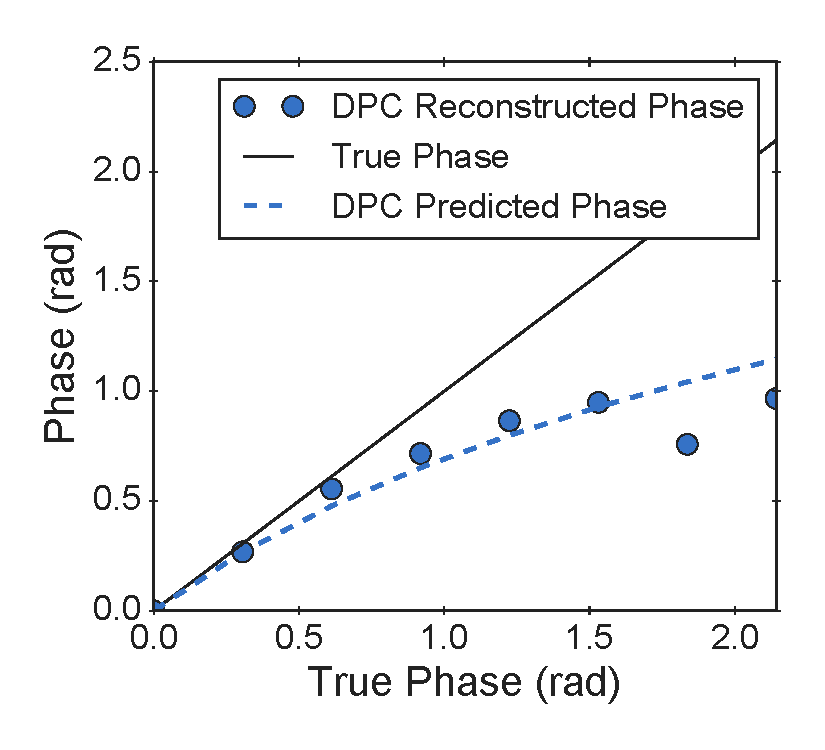
\includegraphics[width=1.0\textwidth]{figures/fig_phase_dpc_validation_2.pdf}
\caption{\label{fig:dpc_validation}
Differential Phase Contrast Reconstruction of a USAF 1951 resolution target printed as a phase object. The DPC linearization becomes less accurate for objects with strong phase ($> 1$ radian) or a strong phase gradient.}
\end{figure}

\subsection{Limitations}
The linearization made by DPC is valid when absorption and phase gradient are small. Practically, DPC will fail to recovery objects which have sharp edges and strong gradients but will successfully recover large phase values which vary slowly (such as a micro-lens array in Fig.~\ref{fig:dpc_cdpchardware})~\cite{Claus2015, chen2018quantitative}. To provide experimental validation of the DPC approximation, we acquired test images for a series of phase targets across a range of physical heights - each having a phase which increases linearly across 9 targets~\cite{phillipstechnical}. These targets were manufactured on a single test slide (Benchmark Technologies), having USAF1951, star targets, a "wedding-cake" structure with three discrete heights. The results are shown in Fig.~\ref{fig:dpc_validation}, illustrating the decreasing validity of the DPC approximation with increasing target height (and target phase). The WOTF prediction can be derived by taking the natural logarithm of the weak-object approximation ($i\phi_{true} \approx 1 + i\phi_{dpc}$), which reveals that the true phase $\phi_{dpc}$ is related to the DPC-recovered phase by the relationship $i\phi_{true}= \texttt{ln}(1 + i\phi_{dpc})$, although this approximation is only valid for a single-scattering model. To place this in context, a typical biological cell monolayer immersed in water will have less than 0.2 radians of phase deviation, making DPC well-suited for these sorts of imaging tasks.

% \subsection{Compatibility with Fluorescence Imaging}
%
% \begin{figure}[tbh]
% \centering
% 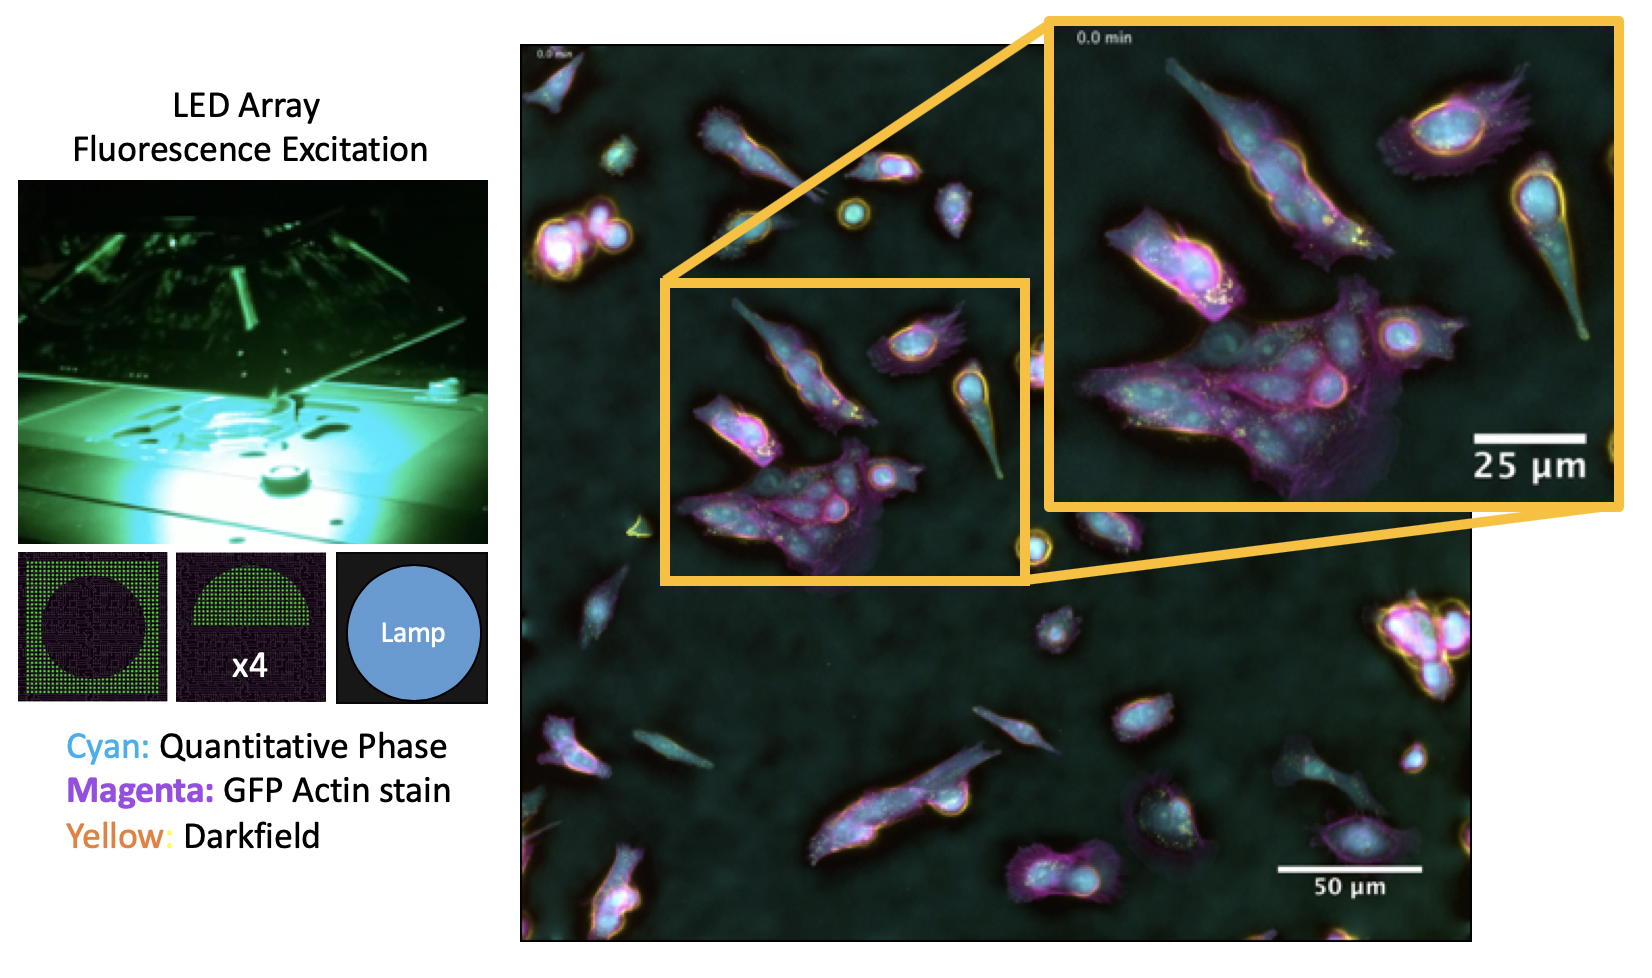
\includegraphics[width=\textwidth]{figures/fig_fabrication_dome_multi.png}
% \caption{\label{fig:dpc_multi} Multi-contrast image of mouse kidney cells using a fluorescent actin stain, single darkfield measurement and four DPC measurements acquired serially using a Nikon TE2000. Dataset was acquired at Analytical and Quantitative Light Microscopy (AQLM) conference in 2017 with help from Justin Taraska (NIH) and Shalin Mehta (MBL)}
% \end{figure}
%
% Because DPC can be implemented in transmission-mode on existing microscopes by the simple addition of a programmable LED array, it is straightforward to perform multi-contrast acquisitions with quantitative phase, darkfield, and wide-field fluorescence microscopy. Figure~\ref{fig:dpc_multi} illustrates a synthesized multi-contrast image which was acquired using a series of 6 images, acquired every 30 seconds. These images are fast to acquire and can be implemented within the existing microscope software using standard software macros.

\section{Single-Shot Quantitative Phase Imaging}\label{sec:phase:cdpc}

\begin{figure}[tbh]
\centering
\includegraphics[width=\textwidth]{figures/fig_cdpc_system.pdf}
\caption{\label{fig:dpc_cdpchardware}
Single-shot color Differential Phase Contrast (\textit{cDPC}) microscopy. a) Installation in Nikon TE300 microscope condenser turret. b) CAD model and image of fabricated \textit{cDPC} insert.c) Optical schematic of a brightfield microscope with a \textit{cDPC} color filter placed at the back focal plane of the condenser in K\"{o}hler configuration. d) Reconstruction: the captured color image is separated into its RGB components, which are then used to recover two unknowns (amplitude and phase) via a well-posed linear deconvolution. The sample is a micro-lens array (Fresnel Technologies 605). }
\end{figure}

To improve temporal resolution of a DPC system without compromising spatial resolution, we propose color Differential Phase Contrast (\textit{cDPC}), which requires only a \emph{single} color image using color-multiplexed source patterns\footnote{This work was performed in close collaboration with Michael Chen (Waller Lab, EECS, UC Berkeley).}. In this method, the source is discretized into three color channels which are used to display three different half-circle source patterns. It is important to note that while the original DPC algorithm presented in \cite{tian2015quantitative} requires 4 images, the proposed method only requires 3, since the 4th source configuration can be synthesized by taking the sum of two images acquired with opposite half-circle illuminations (a synthetic brightfield image) and subtracting that of a 90 degree rotated half-circle source. In early prototypes the color source pattern was implemented in an LED array microscope, which offers many imaging modalities in one platform~\cite{Tian14,zijiMulti,tian2015quantitative,Ma:15,phillips2015multi, Zheng2011, Zheng2013}. More recent work proposed the use of a motion-compensation algorithm to solve for motion between DPC frames, effectivly providing a single-shot phase imaging using computation~\cite{kellman2018motion}. Unlike these methods, however, our proposed configuration does not require a dynamic source, making it possible to use a static multi-color filter placed in the condenser back focal plane, assuming K\"{o}hler illumination. Both configurations simplify hardware and reduce costs significantly as compared to phase contrast or DIC, while providing quantitative phase, which is more general and can be used to synthesize both of the aformementioned methods digitally~\cite{JMI:JMI1027}.

\subsubsection{Hardware Design}
As in conventional DPC, this method requires measurements of the sample illuminated by known asymmetric sources. In \textit{cDPC}, however, we make use of the microscope's existing condenser unit, which has a turret commonly used for phase contrast inserts or DIC prisms. This intermediate plane can usually be accessed easily by removing the mechanical inserts. Taking advantage of this configuration, a simple 3D printed color filter was designed and fabricated that can be placed in the condenser turret of a Nikon TE300 microscope (Figure~\ref{fig:dpc_cdpchardware}a).

The filter prototype consists of Polyethylene Terephthalate (PET) color filters (Lee Filter, Inc.) laser cut to size and installed into a 3D printed insert designed to fit our microscope. Narrow bandwidth illumination filters (e.g. multi-layer coated glass) would separate colors better but suffer from low light throughput and high cost. Therefore, inexpensive and easy-to-cut PET film filters were used; the resulting cross-talk between color channels will be accounted for in post-processing, described below.

The total cost of raw materials is approximately $\$30$ and filters were produced quickly with a 3D printer and laser cutter. One filter is shown in Figure~\ref{fig:dpc_cdpchardware}b; it was installed in the condenser turret of an inverted microscope (Figure~\ref{fig:dpc_cdpchardware}a), replacing one of the removable phase contrast (Ph1, Ph2 or Ph3) inserts.
\subsubsection{Calibration}
\label{Calibration}

Ideally, the color filters would provide perfect separation of the three source patterns into the three-color channels. In reality, both the illumination and camera color channels have cross-talk between the desired wavelengths. To account for this, system calibration is separated into two separate steps: detection-side and illumination-side.

Illumination-side calibration corrects for the relative spectral transmittance of each of the source color filters. The illumination pattern simultaneously encodes three half-circle sources, one each for the RGB color channels. Red and green are opposite half-circles, and blue is rotated by 90 degrees relative to the others. Where the blue and green patterns overlap, a cyan filter (blue + green) was used. Where the blue and red patterns overlap, a purple filter (blue + red) was used. Hence, the final filter design actually contains four quadrants having red, green, cyan and purple filters (see Fig.~\ref{fig:transferfunctions}).

\begin{figure}[tbh]
\centering
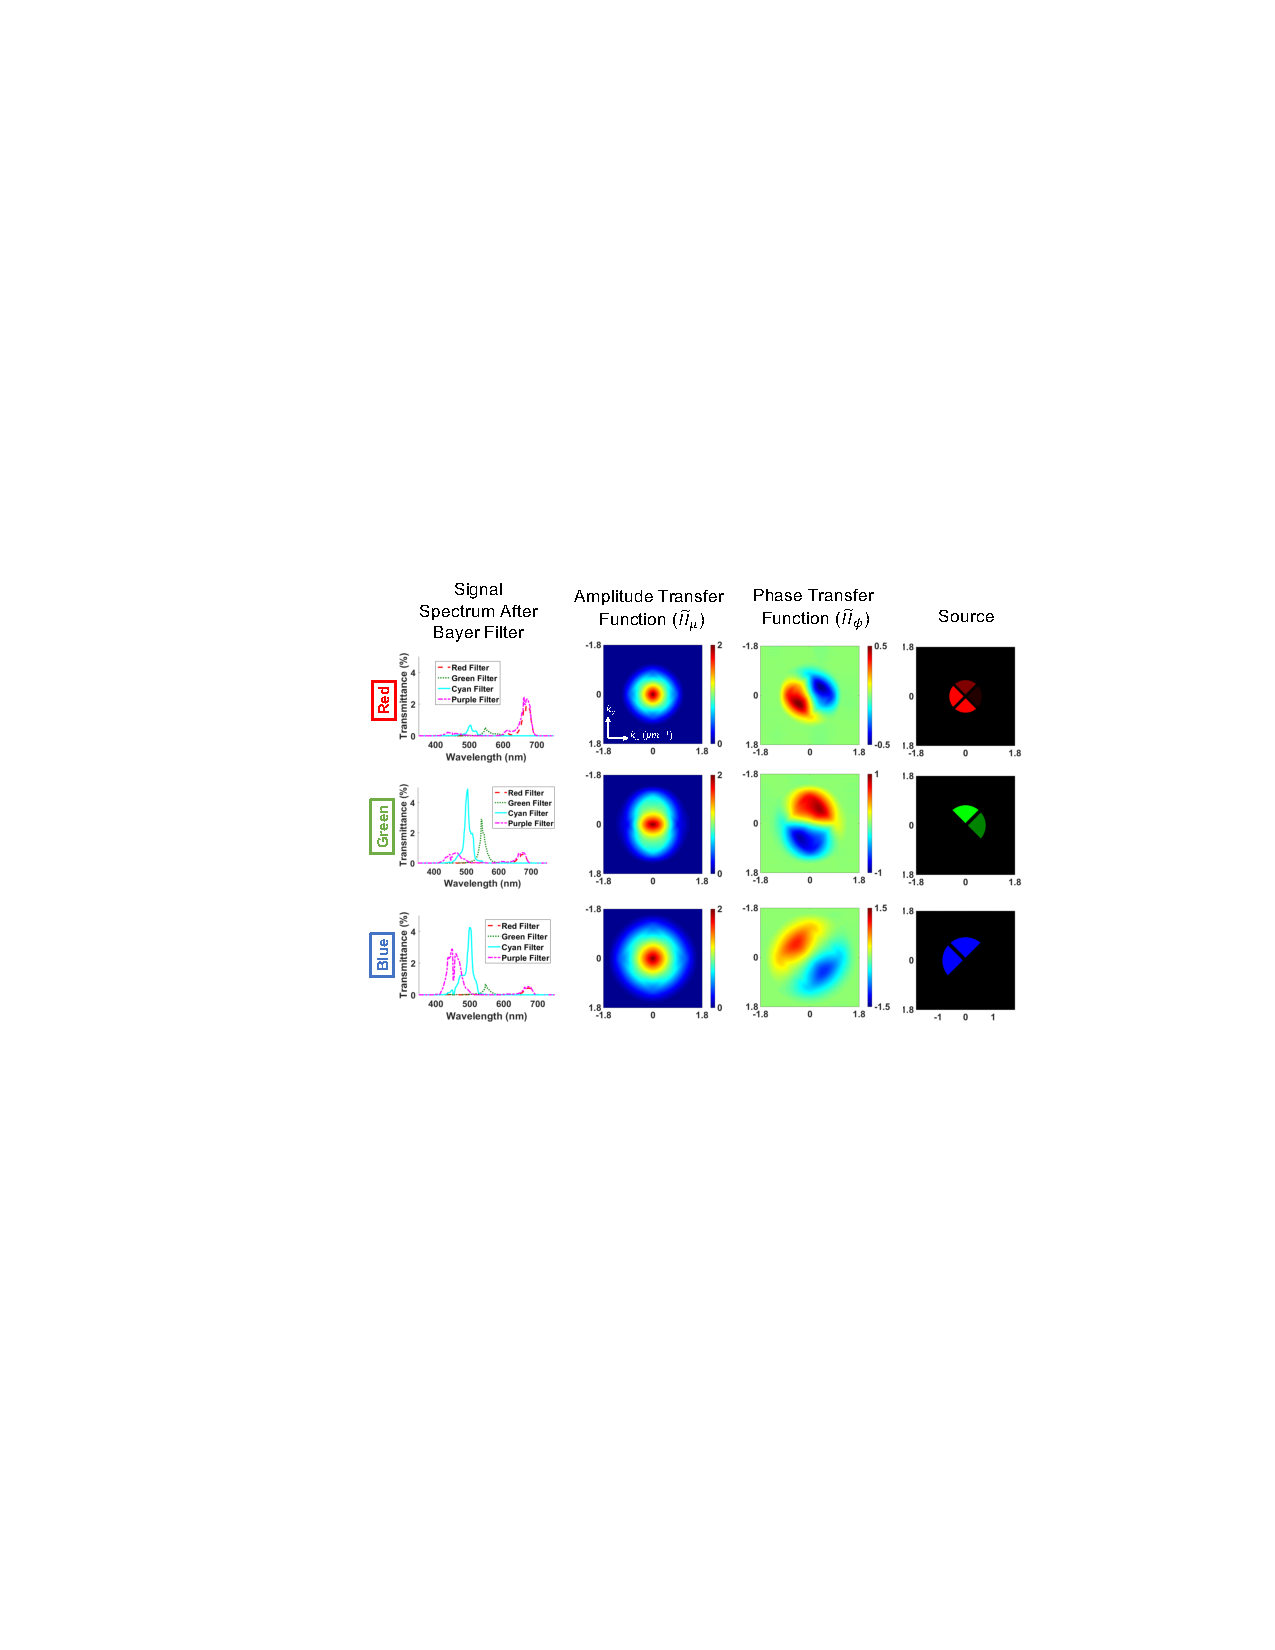
\includegraphics[width=\textwidth]{figures/fig_cdpc_transferfuncs.pdf}
\caption{\label{fig:transferfunctions}
Transfer functions for amplitude and phase contrast in each \textit{cDPC} color channel. Left: Spectral contribution of each illumination filter as captured by the camera's Bayer pattern. The following columns show the components of the amplitude and phase transfer functions in the spatial frequency domain and the source represented in each image.  Bottom row: sum of each column, representing the calibrated and scaled source and the total coverage of amplitude and phase transfer functions, respectively. }
\end{figure}

When filtered by the sensor Bayer pattern, the filter spectrum bases are not orthogonal. This can be seen in the spectra of each PET film after capture with a color camera (left column of Fig.~\ref{fig:transferfunctions}). The result is an undesirable loss of asymmetry in the source that reduces phase SNR. However, it is possible to account for the asymmetry during reconstruction by modeling the source patterns as in Fig.~\ref{fig:transferfunctions}.

Detection-side calibration accounts for spectral cross-talk of the camera color channels. Standard RGB Bayer filters do not provide perfect discrimination between RGB wavelengths but coupling artifacts can be removed by calibration. Given the pixel values from the raw color image with an RGBG Bayer filter ($\vec{I}_r$, $\vec{I}_{g1}$, $\vec{I}_{g2}$, $\vec{I}_b$), it is possible to solve for the decoupled color image ($\vec{I}_R$, $\vec{I}_{G}$, $\vec{I}_{B}$) that would be obtained if the sample were illuminated with a single color, according to the following equation,

\begin{equation}
\label{eq:couplingmatrix}
\begin{bmatrix}
\vec{I}_{r} \\
\vec{I}_{g1}\\
\vec{I}_{g2}\\
\vec{I}_{b}
\end{bmatrix}
 =
 \mat{C}
 \begin{bmatrix}
\vec{I}_{R} \\
\vec{I}_{G}\\
\vec{I}_{B}
\end{bmatrix}.
\end{equation}

\noindent  The matrix $\mat{C}$ is a 4$\times$3 calibration matrix describing the coupling between each color channel. It is generated by filtering the broadband source with each filter independently, then measuring the relative red ($\vec{I}_R$), green ($\vec{I}_G$) and blue ($\vec{I}_B$) read-outs to populate the corresponding column vectors of the $\mat{C}$ matrix. The ratio between the intensities of each flat-field image at each detection channel provides a linear weighting of the contribution of each source to the color measurement. Once $\mat{C}$ has been measured once, it can be used to pre-process all later measurements by solving Eq.~\eqref{eq:couplingmatrix}. This step is important for reducing artifacts in the phase results.

Another important step for \textit{cDPC} is to account for wavelength-dependent changes in phase and spatial frequency. DPC recovers absorption ($\vec{\mu}$) and phase ($\vec{\phi}$) information from intensity measurements. These quantities are defined as:

\begin{equation}
\label{eq:absorption_phase}
\mu = \frac{2\pi}{\lambda_0} \vec{\alpha} \vec{d},\ \phi = \frac{2\pi}{\lambda_0} \vec{n} \vec{d},
\end{equation}

\noindent where $\lambda_0$ is a reference wavelength, $\vec{d}$ is the thickness of the sample, $\vec{n}$ represents refractive index and $\vec{\alpha}$ indicates absorption coefficient. Absorption and phase transfer functions are determined by illumination numerical aperture (NA), objective NA and illumination wavelength~\cite{tian2015quantitative}. In the proposed color-multiplexed DPC method, the transfer functions must also consider the change in wavelength of each color channel. Phase ($\vec{\phi}$) depends on which wavelength is used. By assuming no dispersion in the sample, it is possible to use Eq.~\eqref{eq:absorption_phase} to synthesize phase for any wavelength by simply multiplying the optical path length ($\vec{n}\vec{d}$) by the wave number ($\frac{2\pi}{\lambda_0}$) of a desired reference wavelength $\lambda_0$.

Examining Fig.~\ref{fig:transferfunctions}, it is clear that the absorption transfer functions for each color channel are symmetric low-pass filters. The phase transfer functions, on the other hand, are asymmetric band-pass-like filters with a line of missing frequencies along the axis of asymmetry. By rotating the blue half-circle by 90 degrees relative to the red and green ones, the missing line is filled. The overall amplitude and phase transfer functions for \textit{cDPC} are shown in the last row of Fig.~\ref{fig:transferfunctions}, calculated by summing the absolute values of each color transfer function. As with previous DPC implementations, absorption information loses contrast at high spatial frequencies. Phase has a similar drop-off at high frequencies, but also loses contrast in the low spatial frequency regions. Hence, SNR will be important for accurately recovering low-frequency phase information. The maximum spatial frequency range captured is 2$\times$ the NA of the blue color channel. However, the final resolution using \textit{cDPC} is set by the diffraction limit of green light, since total frequency coverage is set by the maximum spatial frequency which is measured by \textit{two or more} color channels. This comes as an implication of trying to recover two unknowns, amplitude and phase, thus requiring at least two measurements.

\subsubsection{Inverse problem}
Using the forward model developed in Section~\ref{sec:forward}, the \textit{cDPC} inverse problem aims to minimize the difference between the measured color image and that which would be measured, given the estimate of the sample's amplitude and phase:

\begin{equation}\label{eq:objectivefunction}
\begin{split}
\min_{\mu,\phi} \sum_{m=1}^{3}\frac{1}{2} \parallel\tilde{\vec{I}}'(\lambda_m) - \tilde{\vec{H}}_{\mu}(\lambda_m)\cdot \tilde{\vec{\mu}} - \mathrm{i}\cdot\tilde{\vec{H}}_{\phi}(\lambda_m)\cdot \tilde{\vec{\phi}} \parallel_2^2 + \op{R}(\tilde{\vec{\mu}},\tilde{\vec{\phi}}),
\end{split}
\end{equation}

\noindent where $\tilde{\vec{I}}'$ is the spatial frequency spectrum of the background-subtracted intensity, $m$ is the wavelength index and $\op{R}(\tilde{\vec{\mu}},\tilde{\vec{\phi}})$ is a regularization term (typically on the order of $10^{-3}$). This problem is linear and can be solved with a one-step least-square solution (e.g. Wiener deconvolution~\cite{HayesDSP}) or by an iterative algorithm (e.g. gradient descent). The ideal choice of regularizer $\op{R}(\tilde{\vec{\mu}}, \tilde{\vec{\phi}})$ depends on the sample and noise. %Basic $\ell_2$ regularization should be tuned to suppress noise amplification in spatial frequencies that are measured with low-contrast, without destroying sample information at those frequencies. Alternatively, if the sample is sparse (only a few non-zero values), one can use an $\ell_1$ regularizer~\cite{2002_l1_sparcity}. Other types of \textit{a priori} information may be incorporated by appropriate regularization. In the experiments presented here no assumptions on the sample structure were made; However, $\ell_2$ regularization is used to constrain the total energy of the signal and make the problem well-posed. Equation~\eqref{eq:objectivefunction} thus becomes,

\begin{equation}\label{eq:objectivefunction2}
\begin{split}
\min_{\vec{\mu},\vec{\phi}} \sum_{m=1}^{3} \frac{1}{2}  \parallel\tilde{\vec{I}}'(\lambda_m) - \tilde{\vec{H}}_{\mu}(\lambda_m)\cdot \tilde{\vec{\mu}} - \mathrm{i}\cdot\tilde{\vec{H}}_{\vec{\phi}}(\lambda_m)\cdot \tilde{\vec{\phi}} \parallel_2^2 + \gamma_{\vec{\mu}}\cdot \parallel \vec{\mu} \parallel^2_2 + \gamma_{\vec{\phi}}\cdot \parallel \vec{\phi}\parallel^2_2,
\end{split}
\end{equation}

\noindent which remains differentiable and allows us to find the global minimum solution for absorption and phase with a single matrix inversion step. The reconstructed amplitude and phase are obtained using Eq.~\ref{eq:Ha_inverse} and Eq.~\ref{eq:Hp_inverse} as in conventional DPC

\begin{figure}[bth]
\centering
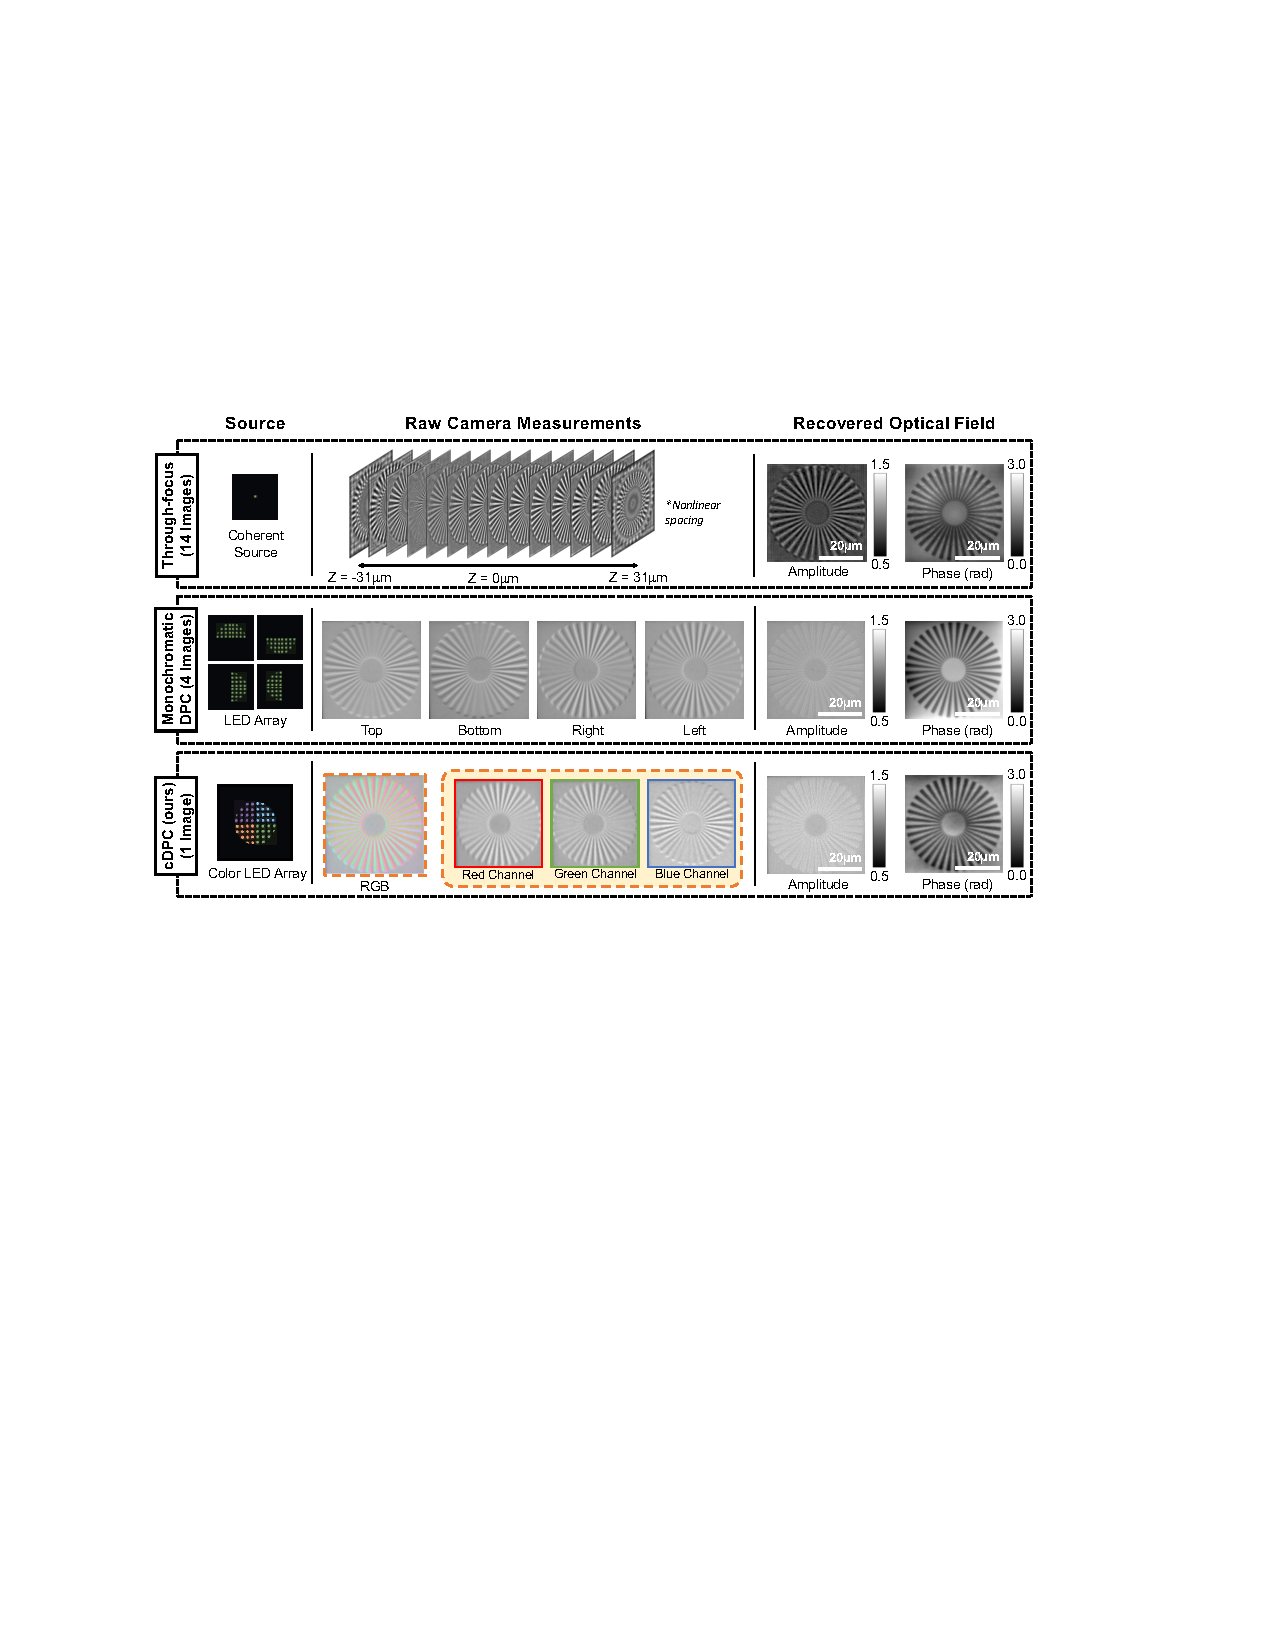
\includegraphics[width=\textwidth]{figures/fig_cdpc_comparison.pdf}
\caption{\label{fig:spatialRes}
Experimental comparison of single-shot \textit{cDPC} with monochromatic DPC and through-focus phase retrieval methods. (Left) Source patterns. (Middle) Raw camera measurements. (Right) Recovered optical field. DPC methods (partially coherent) were acquired using a 20$\times$ 0.4 NA objective lens, while through-focus images (spatially coherent) were captured using 60$\times$ 0.8 NA, in order to ensure equal resolution in all cases.}
\end{figure}

\subsubsection{Validation}

To experimentally validate the proposed \textit{cDPC} method, results were compared with two established QPI methods: monochromatic DPC and through-focus phase retrieval (Fig.~\ref{fig:spatialRes}). For fair comparison, all are implemented on the same Nikon TE300 microscope using illumination generated by an RGB LED array (Adafruit). Each \textit{cDPC} experiment uses a discretized version of the \textit{cDPC} color filter design displayed on the LED array. Monochromatic DPC uses 4 images captured with each of 4 asymmetric source patterns~\cite{zijiMulti}. Through-focus phase imaging uses only the central green LED (for temporal and spatial coherence) while capturing 14 images at different focus depths; phase is then recovered by a nonlinear optimization phase retrieval method~\cite{JingsanSourceRecovery2016}.

Because of the coherent illumination, through-focus phase imaging has 2$\times$ worse resolution than DPC methods. Thus, a 20$\times$ 0.4 NA objective lens was used for DPC methods, but switched to a 60$\times$ 0.8 NA objective for through-focus phase, in order keep resolution equal for all three. Spatial resolution is quantified using a spoke-pattern phase target~\cite{standardphaseresolution2016}.

As can be seen in Fig.~\ref{fig:spatialRes}, the RGB color channel images have similar contrast to the left, right and top images of the monochromatic DPC, as expected. The phase results are also similar, with equivalent spatial resolution. Because the \textit{cDPC} image is captured in one shot with color filters, it has lower SNR than monochromatic DPC and deviates in its low-frequency fluctuations, which have weaker transfer function values. Overall, however, single-shot \textit{cDPC} performs comparably to multi-shot DPC.

Next, the LED array was removed and replaced with the existing illumination pathway. For illumination, a broadband arc lamp light source was used. Alternatively, a high-power blue-phosphor static LED source could be used. The color filter insert shown in Fig.~\ref{fig:dpc_cdpchardware}b was then installed into the condenser turret. Figure~\ref{fig:mosaic} shows amplitude and phase reconstructions from the proposed \textit{cDPC} method with objectives of various magnification. The \textit{cDPC} method is compatible with any standard objective having $ NA_{objective}\leq NA_{illumination}$. If an objective with larger NA than the condenser NA is used, the low frequencies of phase will not be transmitted during image formation (see the phase transfer function in Fig. \ref{fig:transferfunctions}), since phase contrast comes primarily from high-angle illumination. The spatial coherence factor $\sigma$ is often defined as:

\begin{equation}
\sigma = \frac{NA_{illumination}}{NA_{objective}}.
\end{equation}

\begin{figure}[htb]
\centering
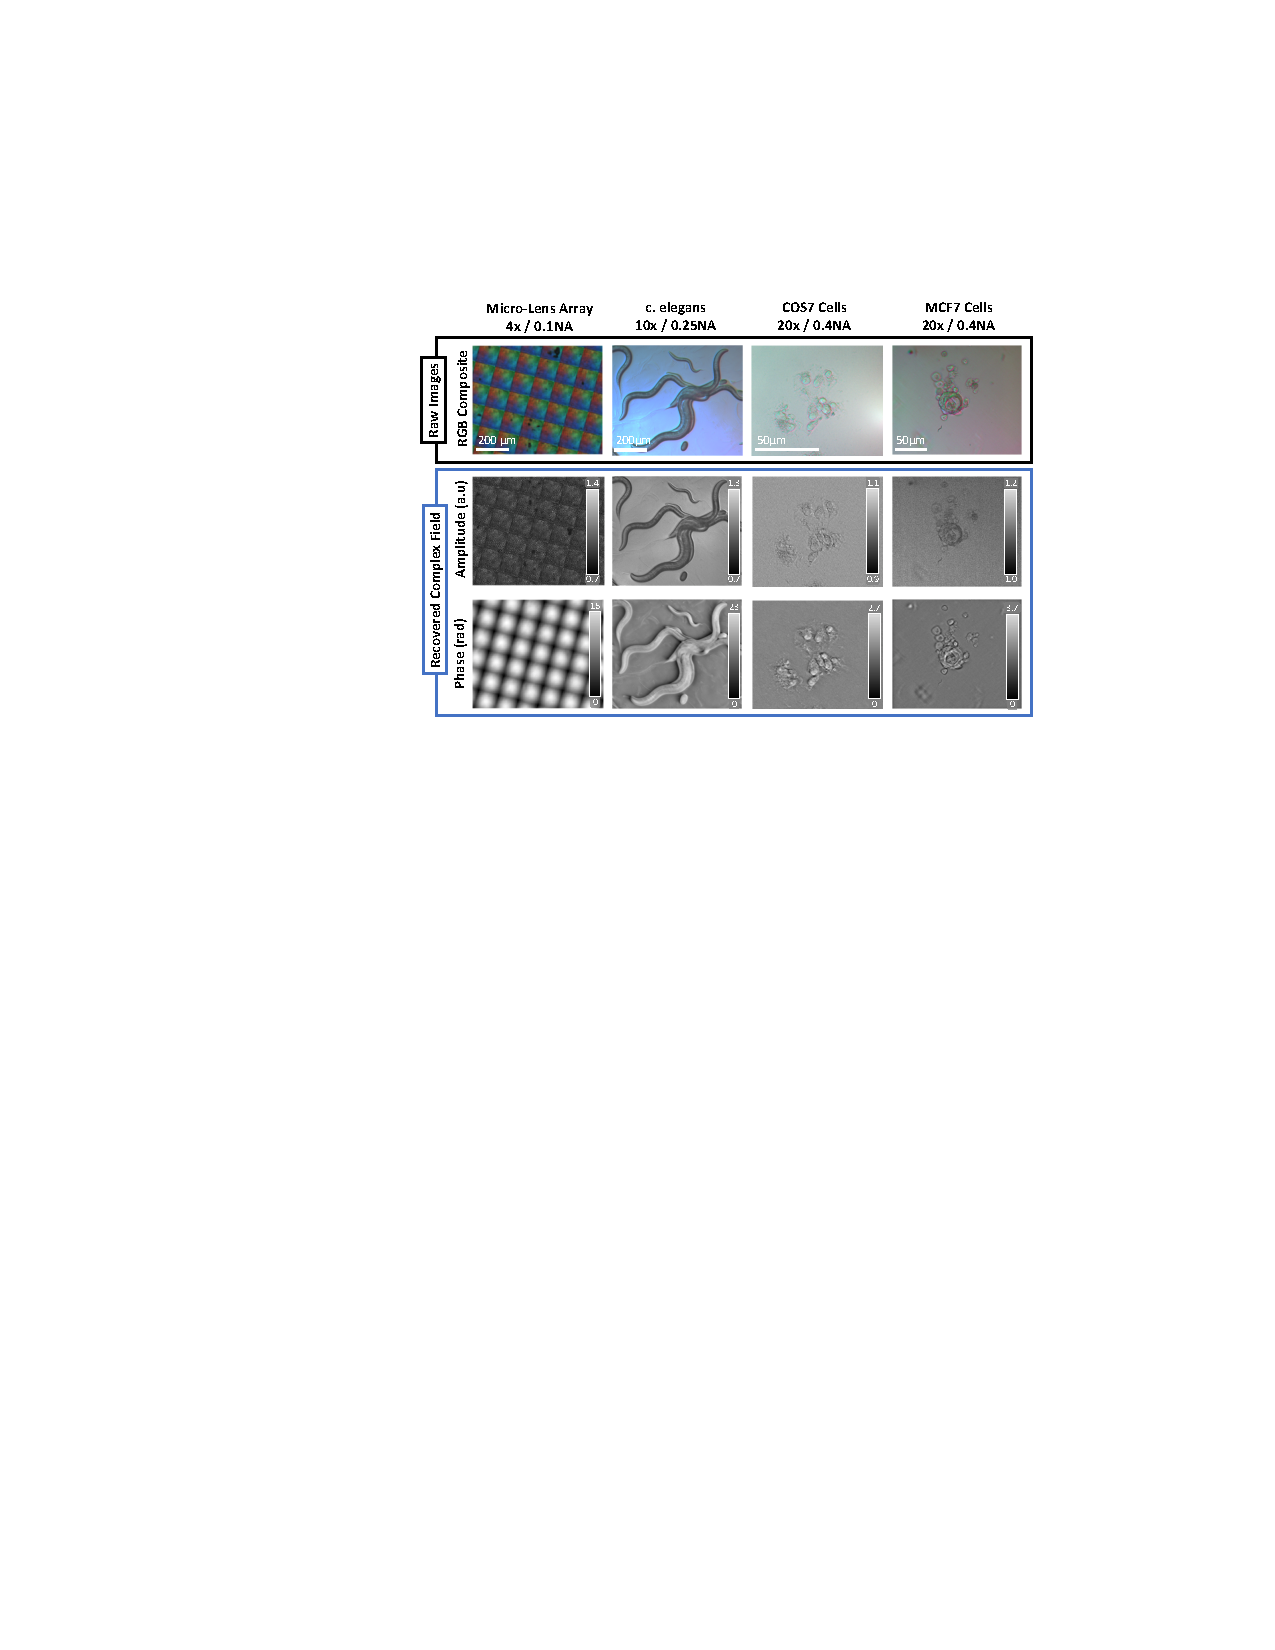
\includegraphics[width=0.9\textwidth]{figures/fig_cdpc_video.pdf}
\caption{\label{fig:mosaic}
Phase and amplitude reconstructions for various samples and magnifications. (First column) Micro-lens array, 4x 0.1 NA. (Second column) Wild-type c. elegans, 10x 0.25 NA. (Third column) HEK 293T cells, 20$\times$ 0.4 NA). (Fourth column) MCF7 cells, 20$\times$ 0.4 NA.}
\end{figure}


\noindent In other words, $\sigma < 1$ will result in reduced phase contrast as compared to the $\sigma \geq 1$ case. The Nikon TE300 microscope used in this study was configured with a 0.53 NA condenser lens. Imaging with a higher objective NA would require high-NA illumination (e.g. by using a domed LED array~\cite{phillips2015multi}). Temporal coherence is set by the bandwidth of the color filters, since these have narrower bandwidth than the camera filters. The full-width-half-maximum (FWHM) bandwidth for the filters used in this study was approximately 50nm, which is similar to the emission spectrum of the LED array used previously~\cite{tian2015quantitative}.

\subsubsection{Temporal Resolution}
Since \textit{cDPC} is single-shot, temporal resolution is set by the camera's frame rate, giving a factor of 4 improvement over conventional DPC. Single-shot methods reduce artifacts due to motion blur and image registration. This can be seen in Fig.~\ref{fig:temporalRes}, where the performance \textit{cDPC} and conventional DPC are compared when imaging a live c. elegans culture. Motion blur is significantly reduced with \textit{cDPC}, since the sample changes rapidly between frames, even at 12.5 frames per second.

\begin{figure}[tbh]
\centering
\includegraphics[width=\textwidth]{figures/fig_cdpc_time.pdf}
\caption{\label{fig:temporalRes}
Experimental demonstration of motion blur reduction with \textit{cDPC} vs. conventional DPC. The \textit{cDPC} method results in significantly reduced motion blur artifacts due to its single-shot acquisition.}
\end{figure}

\subsubsection{Synthesized PhC and DIC Images}

\begin{figure}[tbh]
\centering
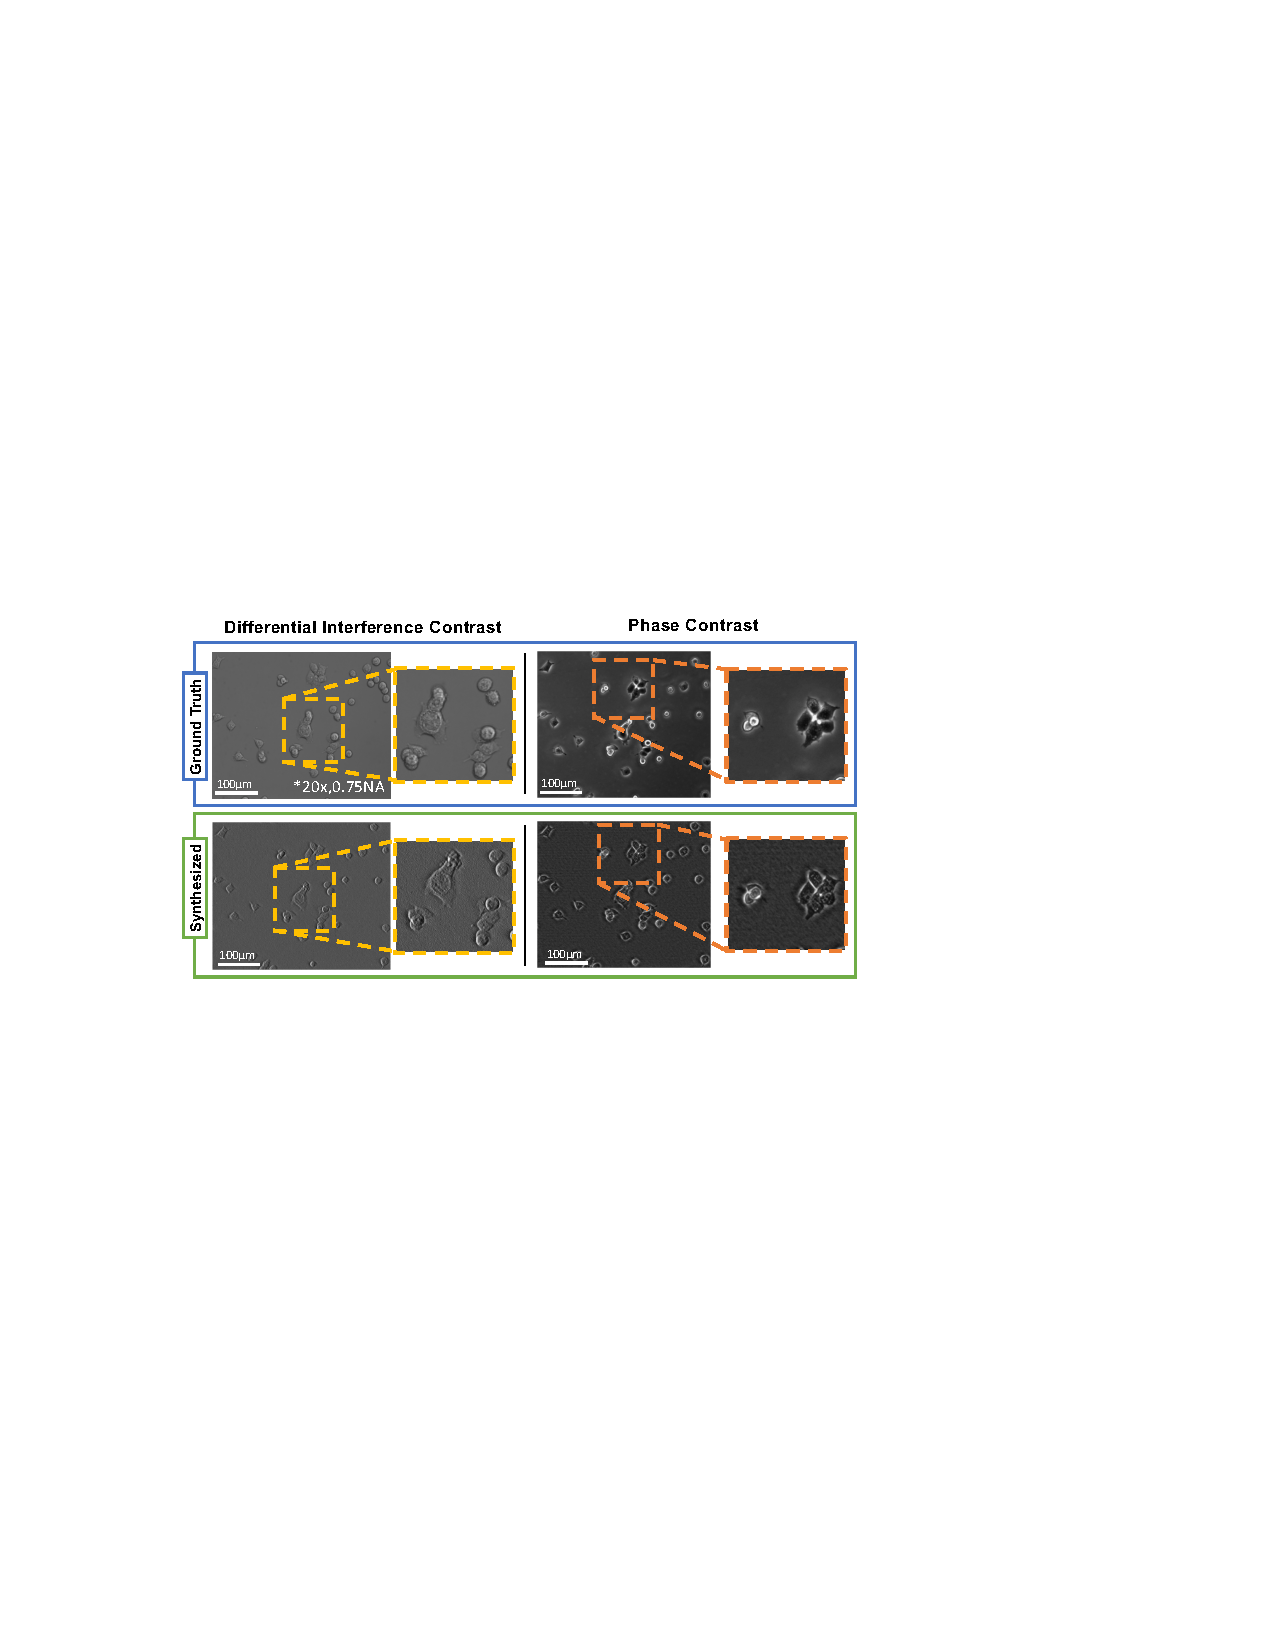
\includegraphics[width=0.8\textwidth]{figures/fig_cdpc_dic.pdf}
\caption{\label{fig:synthDIC_PC}
Comparison of standard DIC and PhC images to their synthesized counterparts from \textit{cDPC}. Ground truth DIC images were acquired using a 20x 0.75 NA objective and phase contrast images using a 20x 0.4 NA PhC objective. \textit{cDPC} images were acquired using a 20x 0.4 NA objective and the filter insert.}\end{figure}

Differential Interference Contrast (DIC) and conventional Phase Contrast (PhC) microscopy are examples of the widespread adoption of phase imaging methods in medicine and biomedical research. Though both methods have gained widespread adoption, optical components required for their implementation remain expensive, and alignment by an experienced user is required for acceptable performance. Both DIC and phase contrast can be described by forward models which produce a qualitative mixture of amplitude and phase images~\cite{zernike1942phase, smithDIC}. Since the forward models of these systems are well known, quantitative phase imaging methods can be used to form these images digitally, mimicking the physical optical system through numerical simulation. Synthesized images from \textit{cDPC}, as well as ground truth DIC and PhC images, are shown in Figure~\ref{fig:synthDIC_PC} to be comparable.

Synthesizing DIC and PhC is of particular use for clinicians and researchers who have been trained to make diagnoses or decisions based on these images. While all QPI methods can be used to synthesize these images, the \textit{cDPC} method is particularly well-suited since it is single-shot, allowing for real-time digital synthesis. In addition, \textit{cDPC} is much cheaper to implement than either DIC or PhC, since it requires only the addition of an inexpensive color filter insert and no specialized objectives. In contrast, DIC prisms and phase contrast objectives (specific to a given NA) can drive up the cost of a microscope significantly.

\subsubsection{Compatibility with Stained and Dispersive Samples}
The \textit{cDPC} method uses color multiplexing to recover complex-field, making an inherent assumption that the sample is both non-dispersive and colorless. Non-dispersive means that the refractive index does not change appreciably with wavelength:

\begin{equation} \label{Eq:nonDispersive}
\vec{\phi}(\vec{n}(\lambda),\vec{d},\lambda) \approx \vec{\phi}(\vec{n}_0,\vec{d},\lambda).
\end{equation}

\noindent This assumption implies that the optical path length ($OPL = nd$) will remain constant for all measurements. The relative phase delay will always vary with $\lambda$ (Eq. \ref{eq:absorption_phase}), but this is accounted for in the \textit{cDPC} algorithm by scaling the transfer functions based on the relative wavelength of each color channel. Unless the dispersion curve is known and the material is assumed to be uniform, one cannot account for dispersive effects in the sample using the proposed algorithm. However, in practice these effects do not corrupt our phase reconstructions results significantly due to relatively small dispersive effects of water across optical wavelengths.

\begin{figure}[tb]
    \centering
    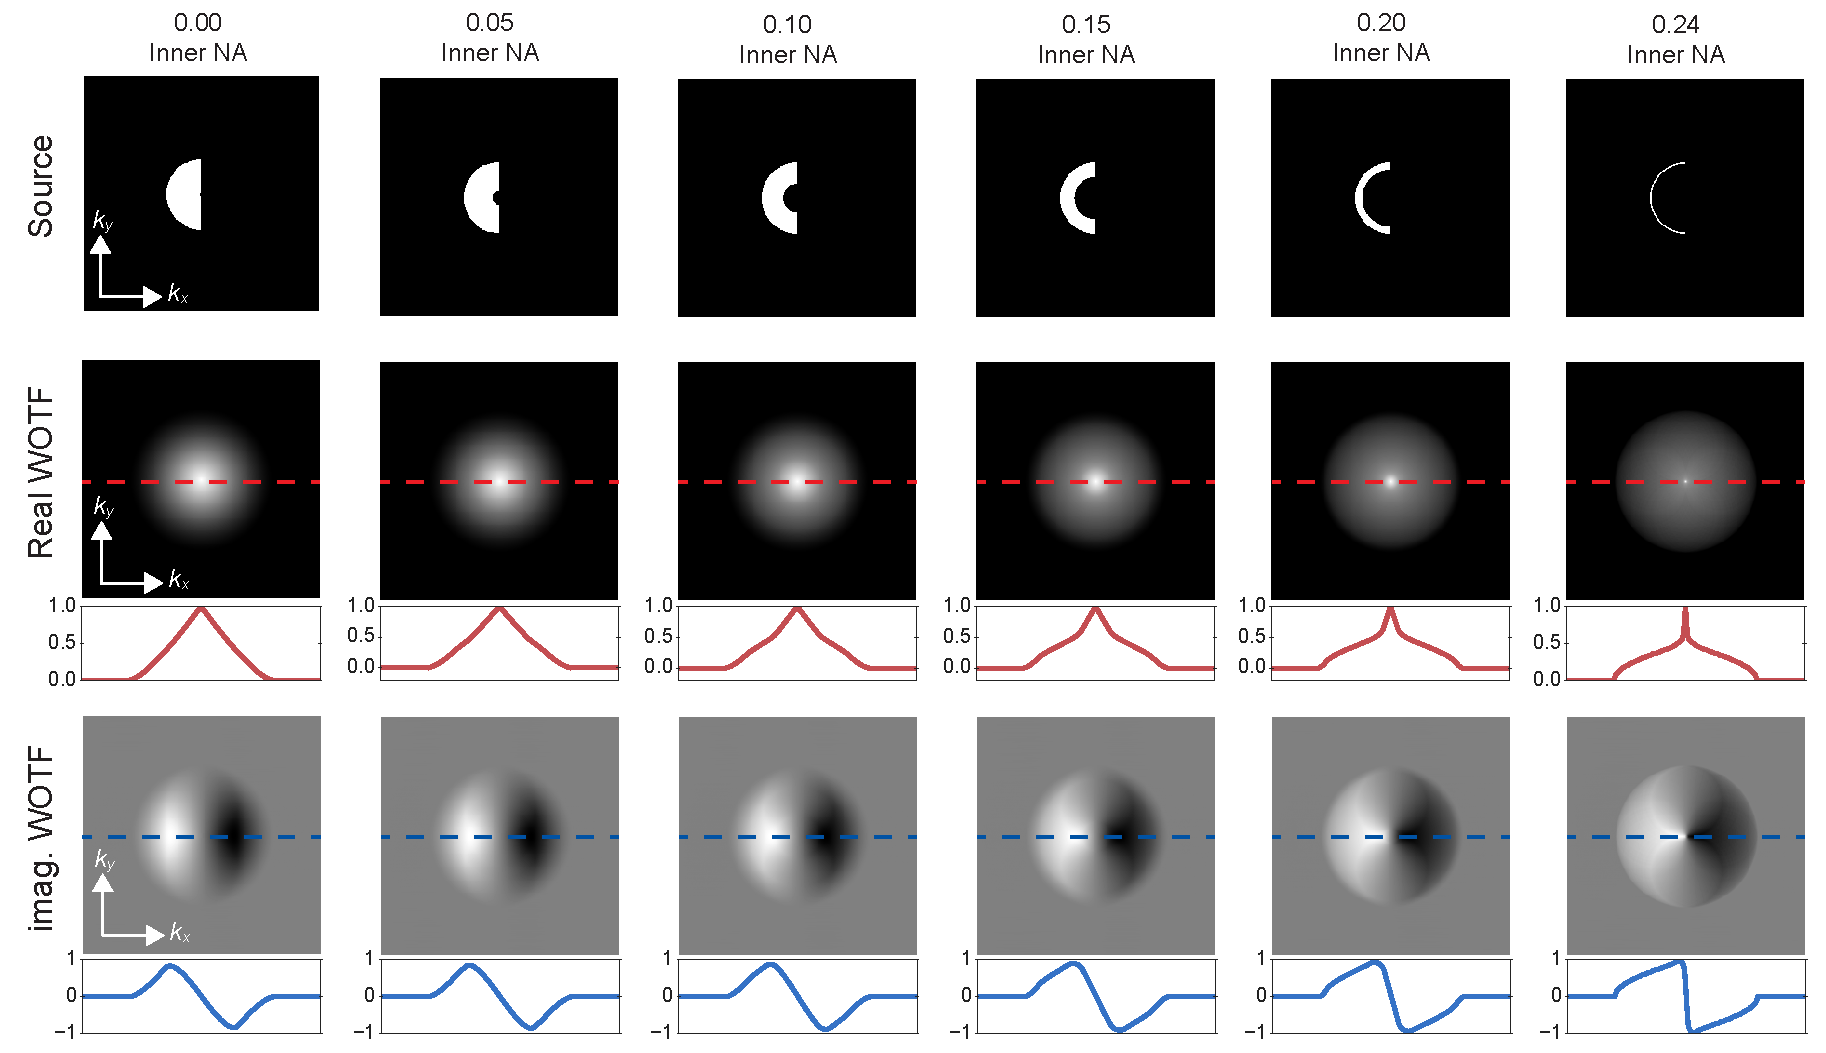
\includegraphics[width=\textwidth]{figures/fig_phase_dpc_opt_transfer.pdf}
    \caption{\label{fig:phase:cavitated_transfer_functions}
    DPC transfer functions for amplitude and phase for a range of source cavitation values. As illumination is removed from the center of the source, the overall spectrum becomes more normalized, leading to higher relative values across the mid-range spatial frequencies. However, signal is simultaneously reduced due to lower light throughput. The trade-off between better conditioning and light throughput depends on the illumination power per pixel (or per led).}
\end{figure}

The second assumption is that the sample is colorless, meaning that the absorption does not have chromatic dependence:
\begin{equation} \label{outEq:monochrome}
\vec{\mu}(\lambda) \approx \vec{\mu}_0.
\end{equation}
\noindent This is generally valid for unstained biological samples, which are transparent. Color variations due to filter transmission coefficients at different wavelengths are present, but can be removed by the calibration procedure described in Section 1.2. Color-dependent absorption, such as that created by stained samples, cannot be recovered and will cause errors in the phase result. In practice, these assumptions limit the applicability of the \textit{cDPC} method to unstained uncolored samples. However, quantitative phase reveals the mechanical structure of the microenvironment with high contrast, which may eliminate the need for staining in many applications.

\begin{wrapfigure}{L}{0.3\textwidth}
  \label{fig:phase:dpc_cavitation}
  \begin{center}
    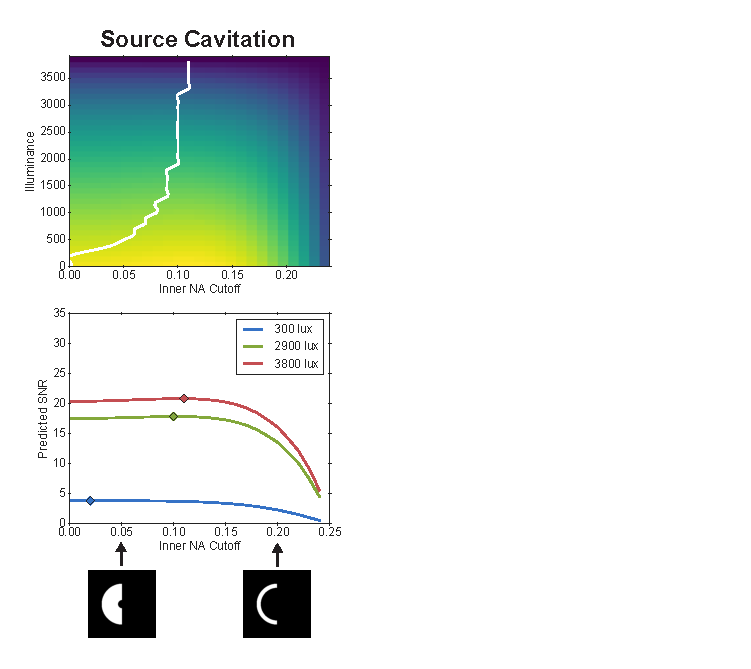
\includegraphics[width=0.3\textwidth]{figures/fig_phase_dpc_optimization_cavitation.pdf}
  \end{center}
  \caption{Expected SNR of DPC reconstructions as a function of source cavitation. Source patterns with no cavitation generally provide nearly-optimal SNR, although a source with cavitation NA of approximately $NA \/ 2$ is optimal for high illuminance values.}
\end{wrapfigure}

\section{SNR Analysis of DPC Phase Recovery Systems}
Differential Phase Contrast linearizes the partially coherent image formation model, enabling the analysis of this system using the noise analysis methods described in Chapter~\ref{ch:introduction}, Section~\ref{sec:intro_noise}. This section will analyze the choice of source pattern and pupil function in the context of our propsed linear noise model, and examine the practical benefit of using a variable number of measurements, variable source diameter, and adding a defocus aberration to the pupil, in terms of reconstruction SNR. Recent works have used learning techniques to explore optimal source designs using non-linear recovery methods (such as an unrolled convolutional network)~\cite{kellman2019physics}) in terms of root-mean-square error (RMSE) - these techniques are non-linear and object dependent, but are compatible with non-linear regluarizers, offering better performance for a specific class of samples with slightly less generality. Our proposed method for optimizing DPC source patterns assumes nothing about the spectrum of the sample, but does not take advantage of non-linear regularization methods.

In the presence of measurement noise (valid for most practical systems) the multi-image DPC forward model described in Eq.~\ref{eq:dpc_forward_model} can be modeled as having an additional additive noise term $\vec{\eta}$:

\begin{equation}
    \label{eq:dpc_forward_model_noise}
    \begin{bmatrix}\tilde{\vec{y}}_1 \\ \tilde{\vec{y}}_2 \\ \tilde{\vec{y}}_3\end{bmatrix} = \begin{bmatrix}\tilde{\vec{H}}_{\mu, 1} & \tilde{\vec{H}}_{\phi, 1}\\ \tilde{\vec{H}}_{\mu, 2} & \tilde{\vec{H}}_{\phi, 2} \\ \tilde{\vec{H}}_{\mu, 3} & \tilde{\vec{H}}_{\phi, 3}\end{bmatrix} \times \begin{bmatrix}\tilde{\vec{\mu}} \\ \tilde{\vec{\phi}}\end{bmatrix} + \vec{\eta}
\end{equation}

\noindent Here $\vec{\eta}$ is modeled as white zero-mean Gaussian noise with variance $\sigma_{\eta}^2$. The goal of the DPC linearization is to facilitate the inversion of the block WOTF matrix; when $\vec{\eta}$ is included in the forward model, this inversion will amplify $\eta$ based on the singular values of the block matrix $\mat{H}$, which are defined by the illumination source $\vec{\tilde{S}}$ and system pupil $\vec{\tilde{P}}$. Here, we explore the design of DPC source patterns $\tilde{S}$ in the presence of additive noise, in terms of reconstruction SNR. The use of a programmable light source such as a LED illuminator enables the easy and efficient programming of $\vec{\tilde{S}}$ simply by changing illumination pattern electronically, making the design space of each source quite large. In this analysis, we explore the use of continuous sources as an approximation of discrete LED sources, as in previous works~\cite{tian2015quantitative, Phillips:17}.

\begin{wrapfigure}[30]{R}{0.3\textwidth}
  \label{fig:phase:dpc_measurement_count}
    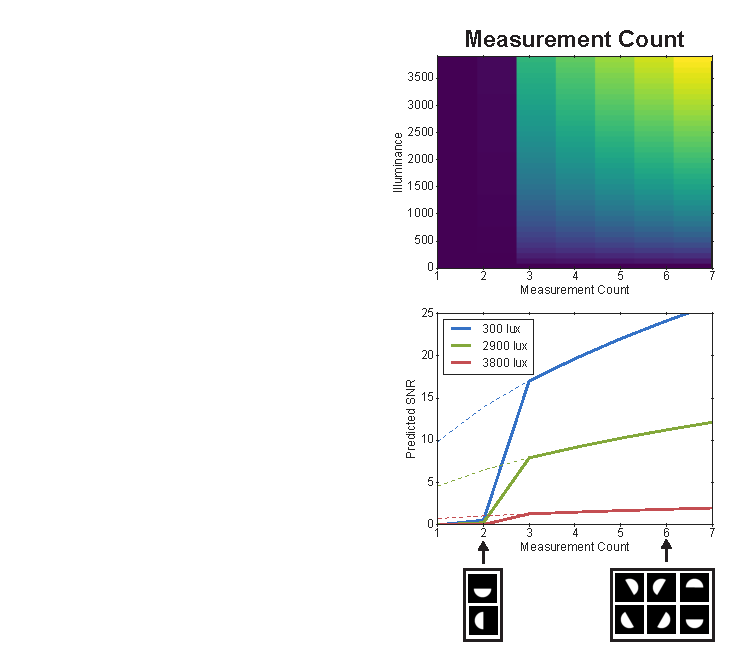
\includegraphics[width=0.3\textwidth]{figures/fig_phase_dpc_optimization_meas.pdf}
  \caption{Expected SNR of DPC reconstructions as a function of measurement count (equidistant angles). SNR increases with the square root of measurement count for more than three DPC measurements, which is the equivalent of averaging measurements under the same noise conditions. For two or less measurements, expected SNR decreases significantly, since there is not enough information to disambiguate phase and amplitude for all frequencies.}
\end{wrapfigure}

The noise amplification of any linear system can be related to the singular values of the forward model by the deconvolution noise factor (DNF, see Chapter~\ref{ch:introduction}, Section~\ref{sec:intro_noise}). In the DPC forward model described in Eq.~\ref{eq:dpc_forward_model_noise}, these singular values may be found by the following relationship~\cite{silvester2000determinants}:

\begin{equation} \label{eq:phase_wotf_singular_values}
\vec{\sigma} = \abs{\frac{tr(\mat{A}^H \mat{A})}{2} \pm \sqrt{\frac{tr(\mat{A}^H \mat{A})^2}{4} - det(\mat{A}^H \mat{A})}}
\end{equation}


Where $\pm$ indicates that both the positive and negative combinations should be included in singular value calculations, $tr(\cdot)$ is the trace and $\det(\cdot)$ is the determinant. Using Eq.~\ref{eq:intro_dnf} to calculate the deconvolution noise factor (DNF), the noise amplification by the DPC inversion process may be estimated using these singular values. Practically, it is necessary to evaluate the DNF within a range of support in the frequency domain, corresponding to the optical bandwidth of the optical system. In addition, the inherent structure of the phase WOTF ($H_{\phi}$) provides very little support near the DC term, which places a lower bound on the support region of the DNF calculation. In this analysis, we evaluate the DNF at all frequencies between 3\% and 97 \% of the optical bandwidth ($2NA_{objective}$), which corresponds to the region where the phase WOTF has more than 5\% of it's maximum value for all angles of a half-circle source and circular pupil.


With this analysis framework, explore the use of a cavitated DPC source in order to improve the conditioning. The cavitated ("C"-shaped) source was previously proposed~\cite{tian2015quantitative} as an alternative to a filled source ("D"-shaped) due to better conditioning of the deconvolution, particularly for low-frequencies of phase. This poor conditioning leads to low-frequency artifacts that often lead to a "halo"-like effect around the sample. Figure~\ref{fig:phase:cavitated_transfer_functions} illustrates the improvement in the phase transfer function at low frequencies for sources with high cavitation. These sources have a overall spectrum which is more flat, corresponding to lower expected noise amplification by the deconvolution process. However, we also expect the additional illumination power provided by center LEDs will also improve SNR, especially in the presence of signal-independent noise (readout or pattern noise). Therefore, we analyze our system across a two-dimensional space of illumination power (defined by illuminance (Lux) at the sample) and source cavitation (defined by the cavitation NA). The goal of this analysis is to determine the optimal cavitation (cavitation NA), given a particular LED source power.

To characterize the relative benefit to using a cavitated source, we simulated measurements performed under various illumination power values (illuminance), which correspond to different measurement SNR values, and evaluated the SNR in the presence of both signal-dependent (shot) noise as well as signal-independent (readout or fixed-pattern) noise sources corresponding to common parameters (The full list of system parameters is provided in Appendix~\ref{sec:appendix:phase}, Section~\ref{sec:appendix:dpc_sys_param}). These illuminance values can be compared to measured source illuminance for LEDs used in this work (Appendix~\ref{sec:appendix:phase}, Section~\ref{sec:appendix:dpc_led_power}). While most DPC sources are discrete, most DPC inversion implementations model the source as continuous to avoid (or average out) LED position calibration error. In this analysis, we adopt the same convention so that our analysis is smooth in terms of cavitation NA.

The results of this analysis are shown in Fig.~\ref{fig:phase:dpc_cavitation}. For per-source LED power of less than 1000 lux, a D-shaped source is optimal due to the additional signal which is provided by the inner LEDs. For brighter sources, an inner NA corresponding to approximately 40-50\% of the objective NA is optimal in terms of SNR, although the SNR improvement is generally less than 5\% compared to a filled-in (non-cavitated) source.

In addition to source cavitation, we can use the same methods to explore other DPC system parameters, including measurement count. The original DPC implementation used 4 measurements~\cite{tian2015quantitative}, but it was later shown that three measurements is sufficient for well-conditioned recovery~\cite{PhillipsChen17cDPC}. To explore this space, we compared using different DPC measurement counts across a range of illumination powers (Fig.~\ref{fig:phase:dpc_measurement_count}). This analysis confirms that reconstructions will fail for less than three measurements, and that using greater than 3 measurements provides improvements which are characteristic of signal averaging ($SNR \propto \sqrt{N}$). This analysis confirms these previous claims and motivates using three DPC measurements in most circumstances (unless signal averaging is needed to improve SNR).

This section provides two examples of optimizing DPC acquisitions using a noise-based analysis. In general, these data indicate that a D-shaped source is still nearly-optimal in most circumstances, with a C-shaped source providing only marginal SNR improvement when using a powerful source. These data also motivate using 3 DPC measurements instead of 4 (spaced equally in angle). Future work could explore the optimal angular distribution of DPC sources, as well as the relative benefit of using diverse DPC sources such as monopole, dipole, or other non-semicircular patterns.

\section{Summary}
Phase imaging enables label-free imaging of samples by revealing variations in refractive index which are naturally present in nearly all biological samples. In this chapter, we described a method for performing quantitative phase imaging using coded illumination (differential phase contrast), which can be implemented easily on a conventional optical microscope. DPC makes use of the weak-object approximation, which linearizes the image formation process, but is less valid for samples having a strong phase gradient (steep or sharp features). Conventional DPC requires 3 or 4 images to recover the full optical field from intensity measurements; Here, we have proposed novel method for performing DPC using only single measurement using a wavelength-multiplexing technique. This method can be implemented using a simple 3D-printed insert (costing less than 30\$ to fabricate), or with a programmable light source such as a LED array. While our method does not match the SNR of conventional DPC using 4 images, it enables significantly higher acquisition frame rates, enabling quantitative phase imaging of fast-moving samples such as \textit{c. elegans} or cells moving through a microfluidic channel. Our method, which we call \textit{cDPC}, also enables the synthesis of conventional phase images, like DIC or phase contrast, since quantitative phase is more general than these qualitative phase measurements. Finally, we proposed a framework for performing DPC source optimization in terms of SNR and explore two areas of source design which reveal optimal illumination patterns across a range of source power. Together, these contributions aim to bring quantitative phase imaging to a wider audience through their simple and inexpensive implementations.
